\documentclass[10pt,a4paper]{article}
\usepackage[utf8]{inputenc}
\usepackage{amsmath}
\usepackage{amsfonts}
\usepackage{amssymb}
\usepackage{graphicx}
\usepackage{color}
\usepackage{float}
\usepackage{gensymb}

\usepackage{listings}
\usepackage[ampersand]{easylist}
\usepackage{setspace}
\usepackage{makeidx}
\usepackage{wrapfig}
\usepackage{etoolbox}

\usepackage{eurosym}
 
\usepackage{fancyhdr}

\usepackage{titlesec}

\setcounter{secnumdepth}{4}

\titleformat{\paragraph}
{\normalfont\normalsize\bfseries}{\theparagraph}{1em}{}
\titlespacing*{\paragraph}
{0pt}{3.25ex plus 1ex minus .2ex}{1.5ex plus .2ex}
 
\pagestyle{fancy}
\fancyhf{}
\rhead{Amsterdam university of applied sciences}
\lhead{Technical Document}
\rfoot{Page \thepage}


\usepackage{draftwatermark}
\SetWatermarkText{}
\SetWatermarkScale{5}

\definecolor{codegreen}{rgb}{0,0.6,0}
\definecolor{codegray}{rgb}{0.5,0.5,0.5}
\definecolor{codepurple}{rgb}{0.58,0,0.82}
\definecolor{backcolour}{rgb}{0.95,0.95,0.92}
\usepackage{listings}
\lstdefinestyle{cstyle}{
    backgroundcolor=\color{backcolour},   
    commentstyle=\color{codegreen},
    keywordstyle=\color{magenta},
    numberstyle=\tiny\color{codegray},
    stringstyle=\color{codepurple},
    basicstyle=\footnotesize,
    breakatwhitespace=false,         
    breaklines=true,                 
    captionpos=b,                    
    keepspaces=true,                 
    numbers=left,                    
    numbersep=5pt,                  
    showspaces=false,                
    showstringspaces=false,
    showtabs=false,                  
    tabsize=2
}
\lstset{ %
    backgroundcolor=\color[RGB]{250,250,250},   % choose the background color; you must add \usepackage{color} or \usepackage{xcolor}
    basicstyle=\ttfamily,        % the size of the fonts that are used for the code
    breakatwhitespace=false,         % sets if automatic breaks should only happen at whitespace
    breaklines=true,                % sets automatic line breaking
    captionpos=b,                    % sets the caption-position to bottom
    commentstyle=\color[RGB]{0,128,0},    % comment style
    extendedchars=true,              % lets you use non-ASCII characters; for 8-bits encodings only, does not work with UTF-8
    frame=lines,                    % adds a frame around the code
    keepspaces=true,                 % keeps spaces in text, useful for keeping indentation of code (possibly needs columns=flexible)
    keywordstyle=\color{blue},       % keyword style
    language=C,                 % the language of the code
    numbers=left,                    % where to put the line-numbers; possible values are (none, left, right)
    numbersep=10pt,                   % how far the line-numbers are from the code
    numberstyle=\color[RGB]{50,50,50}, % the style that is used for the line-numbers
    rulecolor=\color{black},         % if not set, the frame-color may be changed on line-breaks within not-black text (e.g. comments (green here))
    showstringspaces=false,          % underline spaces within strings only
    showtabs=false,                  % show tabs within strings adding particular underscores
    stepnumber=1,                    % the step between two line-numbers. If it's 1, each line will be numbered
    stringstyle=\color[RGB]{128,0,128},     % string literal style
    tabsize=2,                       % sets default tabsize to 2 spaces
    title=\lstname                   % show the filename of files included with \lstinputlisting; also try caption instead of title
}
\renewcommand{\lstlistingname}{Code}% Listing -> Algorithm
\renewcommand{\lstlistlistingname}{Codes}

\graphicspath{ {./images/} }

\begin{document}
\begin{titlepage}
    \centering
    \vfill
    {\Large

    Swarming Module\\

   
    {\small Technical Document}\\
    {\small Version 1.0}\\
    {\small \today}\\
        
        \vskip2cm
        {\small M. van Wilgenburg, W. Mukhtar, E. van Splunter, M. Siekerman, T. Zaal and M. Visser}\\
    }    
    \vfill
%    \includegraphics[width=1\textwidth]{WireS4}
    
    \vfill
    \vfill
\end{titlepage}

\newpage

\listoffigures
\newpage

\listoftables
\newpage

\tableofcontents
\newpage

\section{Abstract}

\section{Introduction}
This document describes the technical aspect of the "Swarming Module". This module is developed by students of the Amsterdam University of Applied sciences in collaboration with the Delft University of Technology.   This project is a part of a running research program that is looking into the benefits of swarming compared to "standard" approaches, which would be one bigger and more complex robot doing all the work. Finally this program looks at the applications swarming might have on Mars. 

This project contributes to the program by developing a so called "Swarming Module". This module will allow units in a swarm to determine the relative location to one another. When the units know their relative location, multiple complex tasks can be achieved like: path finding, payload transfer from one unit to another, autonomous recharging, and much more. 

\subsection{Swarming}
The term "Swarming" is still a wide concept which is not well defined. However most people agree the following criteria should be met before a group of robots can be defined as a swarm:

\begin{itemize}
	\item Autonomy - It is required that the individuals that make up 	the swarm-robotic system are autonomous robots. They are able to 		physically 		interact with the environment and affect it\cite{swarmintelligence}.
	\item Large number - A large number of units is required
	as well, so the cooperative behavior (and
	swarm intelligence) may occur. The minimum number
	is hard to define and justify. The swarm-robotic
	system can be made of few homogeneous groups of
	robots consisted of large number of units. Highly heterogeneous
	robot groups tend to fall outside swarm
	robotics.\cite{swarmintelligence}
	\item Limited capabilities - The robots in a swarm
	should be relatively incapable or inefficien on their
	own with respect to the task at hand.\cite{swarmintelligence}
	\item Scalability and robustness - A swarm-robotic
	system needs to be scalable and robust. Adding the
	new units will improve the performance of the overall
	system and on the other hand, loosing some units will
	not cause the catastrophic failure.\cite{swarmintelligence}
	\item Distributed coordination - The robots in a swarm
	should only have local and limited sensing and communication
	abilities. The coordination between the
	robots is distributed. The use of a global channel for
	the coordination would influence the autonomy of the
	units.\cite{swarmintelligence}
\end{itemize}

The swarming module provides the information so the last criteria 'Distributed coordination' can be met. The specifications must be formulated so they meet the criteria of "Large numbers", and "Scalability and robustness". It would be preferable to make the swarm endlessly scalable, however hardware limitations will probably hinder this. 

\subsection{Specifications}
Before the features of the Swarming module are specified, swarming itself should be specified further. In section 1 of the research document this is done by creating a set of realistic scenarios. From this specifications like: minimal distance, maximal distance, maximum number of units, and precision are derived. These specifications are summarised in Table \ref{smrange} and Table \ref{specunits}. 

\begin{table}[h]
\centering
\resizebox{\textwidth}{!}{%
\begin{tabular}{|l|l|l|}
\hline
                     & \textbf{Close range (0 - 3 m)} & \textbf{Long range (3 - 25 m)} \\ \hline
Dead zone distance    & 0,015 meters                   & 2 meters                      \\ \hline
Deviation (distance) & +/- 9\%                         & +/- 1 meter                   \\ \hline
Angle Resolution     & 45\%                            & -                             \\ \hline
Update frequency     & 40 Hz                           & 1 Hz                           \\ \hline
\end{tabular}%
}
\caption{Swarming localization specifications}
\label{smrange}
\end{table}

\begin{table}[h]
\centering
\resizebox{\textwidth}{!}{%
\begin{tabular}{|l|l|l|l|l|}
\hline
 & \textbf{minimum} & \textbf{maximum} & \textbf{maximum (close range)} & \textbf{Preferred (demonstration)} \\ \hline
Number of Units & \multicolumn{1}{c|}{3} & \multicolumn{1}{c|}{$\infty$} & \multicolumn{1}{c|}{130} & \multicolumn{1}{c|}{6 to 12} \\ \hline
\end{tabular}%
}
\caption{Specifications number of units}
\label{specunits}
\end{table}


The choice is made to divide the the specifications for localization into two categories: Close range, and long range. This choice was made because at close range more precision precision is needed to prevent the robots from crashing into each other. While at long range the localization will be used not to loose the swarm. The maximum number at close range is derived from the theoretical number of units that can physically fit in a 3 meter radius. And the preferred number of units for demonstration purpose is used to set a goal for the project. For further clarification how these specifications are determined see chapter one of the research document.

\section{Research}
This section will a summary of the findings during the research phase. For the full research done during this project we refer to the "Research Document". \\
The research is split up in the following different subjects: Localization, Hardware communication protocol, Software communication protocol.

\subsection{Localization}
This section will cover the following subjects: Relative distance measurement, and Relative angle measurement. With these two variables the relative location of other units can be derived. 

\subsubsection{Relative distance}
Before any calculations can be done to derive the angle of other units a distance must first be determined. The first choice that has to be made is what type of signal is used to do this. The most commonly used type of signal to measure distance are radio waves, which propagate with the speed of light. Hardware to measure these  signals over short distances, would require clock-speeds of in the GHz, hence be expensive and unstable. Therefore the choice is made to use acoustic signals to measure the distance. This drastically lowers the requirements for the hardware that detects the signal.

Now that this is established there are still two ways to implement a distance measurement. These are: Time of flight (TOF), and Received signal strenght (RSSI). During experiments (found in section 4.3 of the Research document) we found that the received amplitude of the acoustic signal was not proportional to the distance. We also found that the signal was still well defined over the specified distance of three meters. Because of this the signal can be detected and used for TOF.

A system is proposed that combines the two signals (radio and acoustic) in one system. Swarming modules each get their place in time to send their acoustic signal. At the moment the module starts sending the acoustic signal, he sends a message over the radio communication channel saying "im going to send my signal", the radio signal arrives close to instantly compared to the acoustic signal. At this point all the other modules start their timers, and stop them when the acoustic signal arrives a few moments later. The distance can now be calculated to multiply the time with the speed of sound.

\subsection{Relative angle}
Determining the relative orientation with respect to each other can be done in various ways. some methods involve larger limitations than others. In general angular measurements are done using goniometric equations. It was found that calculating the angle with a single measuring point on every swarming module has one big problem. Because geometric functions are used to calculate the angle, there will always be two solutions to the equation (see figure \ref{circle} and section 3.1.1 of the Research document). To solve this the units would have to move and recalculate again to get the right answer. This would limit the units in their movement and functionality and is non desirable.
\begin{equation}
Because\ Xp = Xq,\ cos(-\alpha) = cos(\alpha)\ applies
\end{equation}

\begin{equation}
Because\ Yq = -Yp,\ sin(-\alpha) = -sin(\alpha)\ applies
\end{equation}


To solve this problem a system is proposed with three or more acoustic receivers with a predefined distance between them. Using the difference in time and the predefined distance, the angle can be calculated with only one solution. This method is shown in figure \ref{trigonometry}.

\begin{figure}[H]
\centering
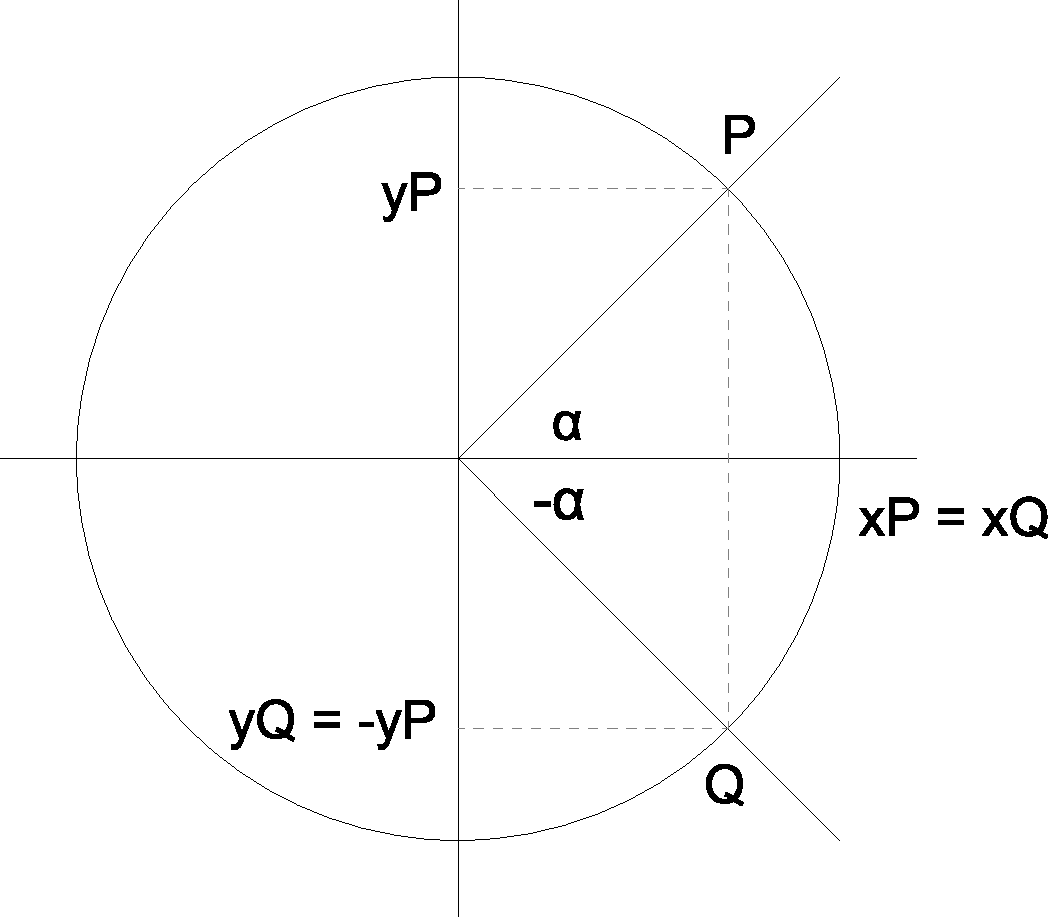
\includegraphics[width=0.7\textwidth]{Cirkel.pdf}
\caption{Unit circle where points P and Q are mirrored on the X-axes}
\label{circle}
\end{figure}



\begin{figure}[H]
\centering
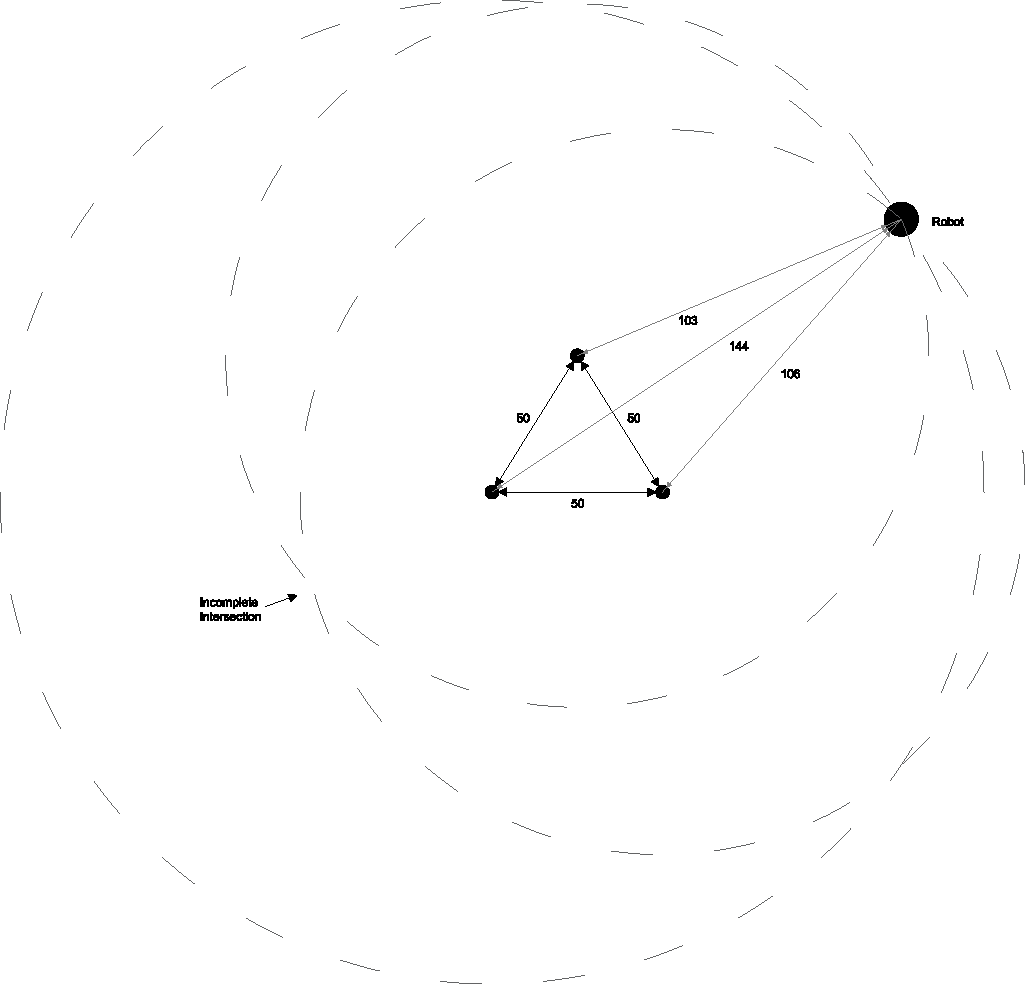
\includegraphics[width=1\textwidth]{trigonometry.pdf}
\caption{Angle determination using trigonometry}
\label{trigonometry}
\end{figure}

\subsection{Demodulation methods}
As talked about before the signal will be modulated and demodulated to introduce a reference point in the signal. This reference point is used to  determine the exact time the signal has travelled. Also the incoming signal from the microphone will suffer from noise and interference. Because of this the demodulator should be noise resistant. Also its part of the specification of the swarming module that it should be a robust system. Therefore the use of high clock micro controllers and complicated software are not preferred.

Project members had experience with frequency demodulation using an analog PLL, and were confident this could be easily tested relatively quick. This will be discussed in the next subsection.

\subsubsection{Analog Phase locked loop}
As discussed in section 9.3 of the technical design a PLL is used to demodulate the signal. A window comparator translates the VCO-in voltage into binary code. To test the precision in time a test set-up was build. Two xmega128a4u were used, one for the demodulator side and one for de modulator side see figure \ref{fig:testup} . During tests the PLL was able to lock on the acoustic signal from a maximum distance of 4 meters which is well within the specification of 3 meters.  The PLL was also able to demodulate the FSK signal at this range. So now the reference point could be identified by the demodulator.

\begin{figure}[H]
   \centering
   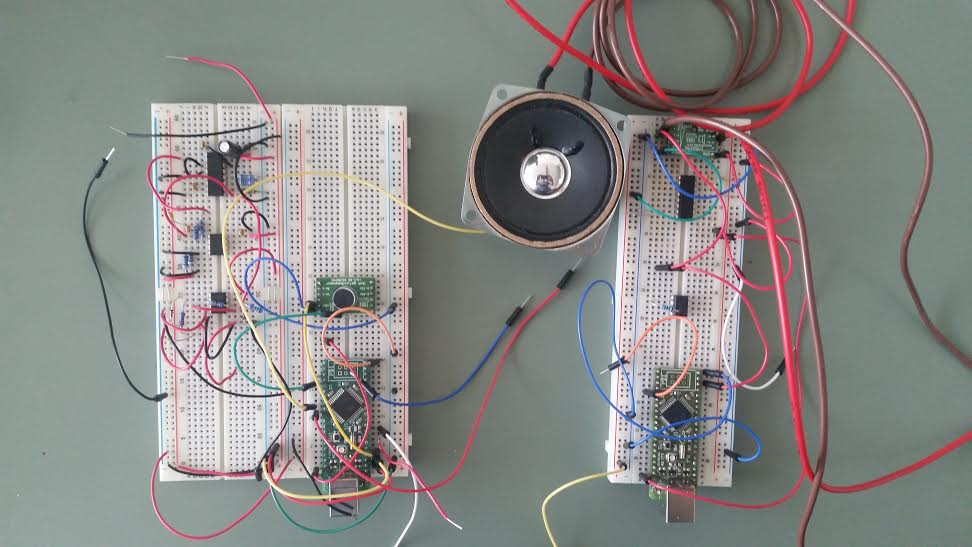
\includegraphics[width=\textwidth]{testopstelling.jpg}
   \caption{Test set-up, the right breadboard is de modulator with a speaker, the left breadboard is the demodulator with an microphone and the PLL}
   \label{fig:testup}
\end{figure}

% Please add the following required packages to your document preamble:
% \usepackage{graphicx}
\begin{table}[h]
\centering
\resizebox{\textwidth}{!}{%
\begin{tabular}{|l|l|l|l|l|l|l|l|l|l|l|}
\hline
Measure point & 1       & 2       & 3       & 4       & 5       & 6       & 7       & 8       & 9       & 10      \\ \hline
0,1m        & 3115769 & 3011495 & 3048980 & 3048133 & 3113623 & 3049715 & 3112041 & 3114898 & 3041495 & 3115769 \\ \hline
1m          & 3112100 & 3012334 & 3102004 & 3159832 & 3068347 & 3123548 & 3110398 & 3119478 & 3062395 & 3119325 \\ \hline
3m          & 3130596 & 3105236 & 3120056 & 3125069 & 3140686 & 3101498 & 3130295 & 3049821 & 3101956 & 3120549 \\ \hline
\end{tabular}%
}
\caption{Measured times in clock pulses, pre scaler is set to 1024 }
\label{measuretime}
\end{table}

The modulator and the demodulator are connected with a wire. The modulator sends a bit when it starts to send the acoustic signal. This bit interrupts the demodulator which starts a timer. When the reference point in the acoustic signal is detected by the PLL the windows comparator sends a binary '1' to the micro-controller which stops the timer. The timer values were then printed in a terminal and are documented in table \ref{measuretime} The measured times are printed in clock pulses with a pre-scaler of 1024. At close range the measured times seem the most stable. However some big deviations of around 500.000 clock pulses still exist. When these times are used to calculate the distance this would mean a deviation is distance of around 5 meters, which is unacceptable. The digital part of the demodulator is tested by connecting a frequency generator to it and observing the time deviation. The time deviation was at a maximum of 200 clock pulses, which is acceptable. The timing deviation is clearly created by the PLL. In section 9.3 of the research document was stated that the PLL would introduce a constant time deviation because of the RC time introduced by the loop filter. We suspect that the reason for the deviation is caused by the window comparator. The time the windows comparator takes to switch from 0 to 5 volt might deviate, which in turn causes the deviation in time. We have not found a way to test or measure this assumption though. Because if this problem the analog PLL approach is not usable for this project.

\subsubsection{Demodulating with a Microproccessor}
Its been established that the analog solution does not meet the criteria. The other option is to process the signal digitally, with an microprocessor. The ADC of the Xmega contain an comparator. This can be used to detect how many times the incoming signal goes trough a certain threshold. From this information the frequency can be derived.

\subsection{Acoustic Sensing}
In this section the behaviour of acoustic signals will be researched. This was done in real life experiments using a microphone, speaker and scope to analyse the received signals. During experiments the following points where analysed:

\begin{itemize}
\item Sound has to spread in every direction (omnidirectional).
\item The received acoustic signal has to be well defined within a minimal distance of 3 meters.
\item What frequency shows the best results.
\end{itemize}

More details about the experiment and the setup are shown in section 4 of the Research document. The first experiment had the speakers facing the microphone directly, this was clearly the best situation, higher frequencies showed higher amplitude and the signal was well defined. However the most ideal situation would be for one speaker to be omnidirectional instead of having to use multiple speakers.  \\
Another test was done with the speaker and microphone both facing upwards. It was observed that higher frequency sound (around 5kHz) becomes more directional. The best results were achieved around 3 - 4 kHz, this was the point where the highest amplitude was achieved and the minimum distance of three meters was easily met.

\newpage




\section{Functional specification}
This chapter describes the functional design of the swarming module. An overview of the swarming module is given in figure \ref{overall}. The module is designed in such a way that it is modular. This module can be placed on an object (i.e. a robot) and can be used by the object to send and receive relevant information about other in-range swarming modules.

This chapter discusses the following subjects:
\begin{itemize}
\setlength\itemsep{0em}
\item Swarming module
\item Power supply and safety
\item Central operating unit
\item Wireless communication module
\item Relative orientation sensor
\item Orientation sensor
\item Localisation sensor
\end{itemize}

\subsection{Swarming module}
The overall design of the swarming module is shown in figure \ref{overall}. Each block of the overall design is described in the following figures. The central operating unit is at the hearth off the swarming module, and takes care of the localization algorithm.
\begin{figure}[h]
  \centering
      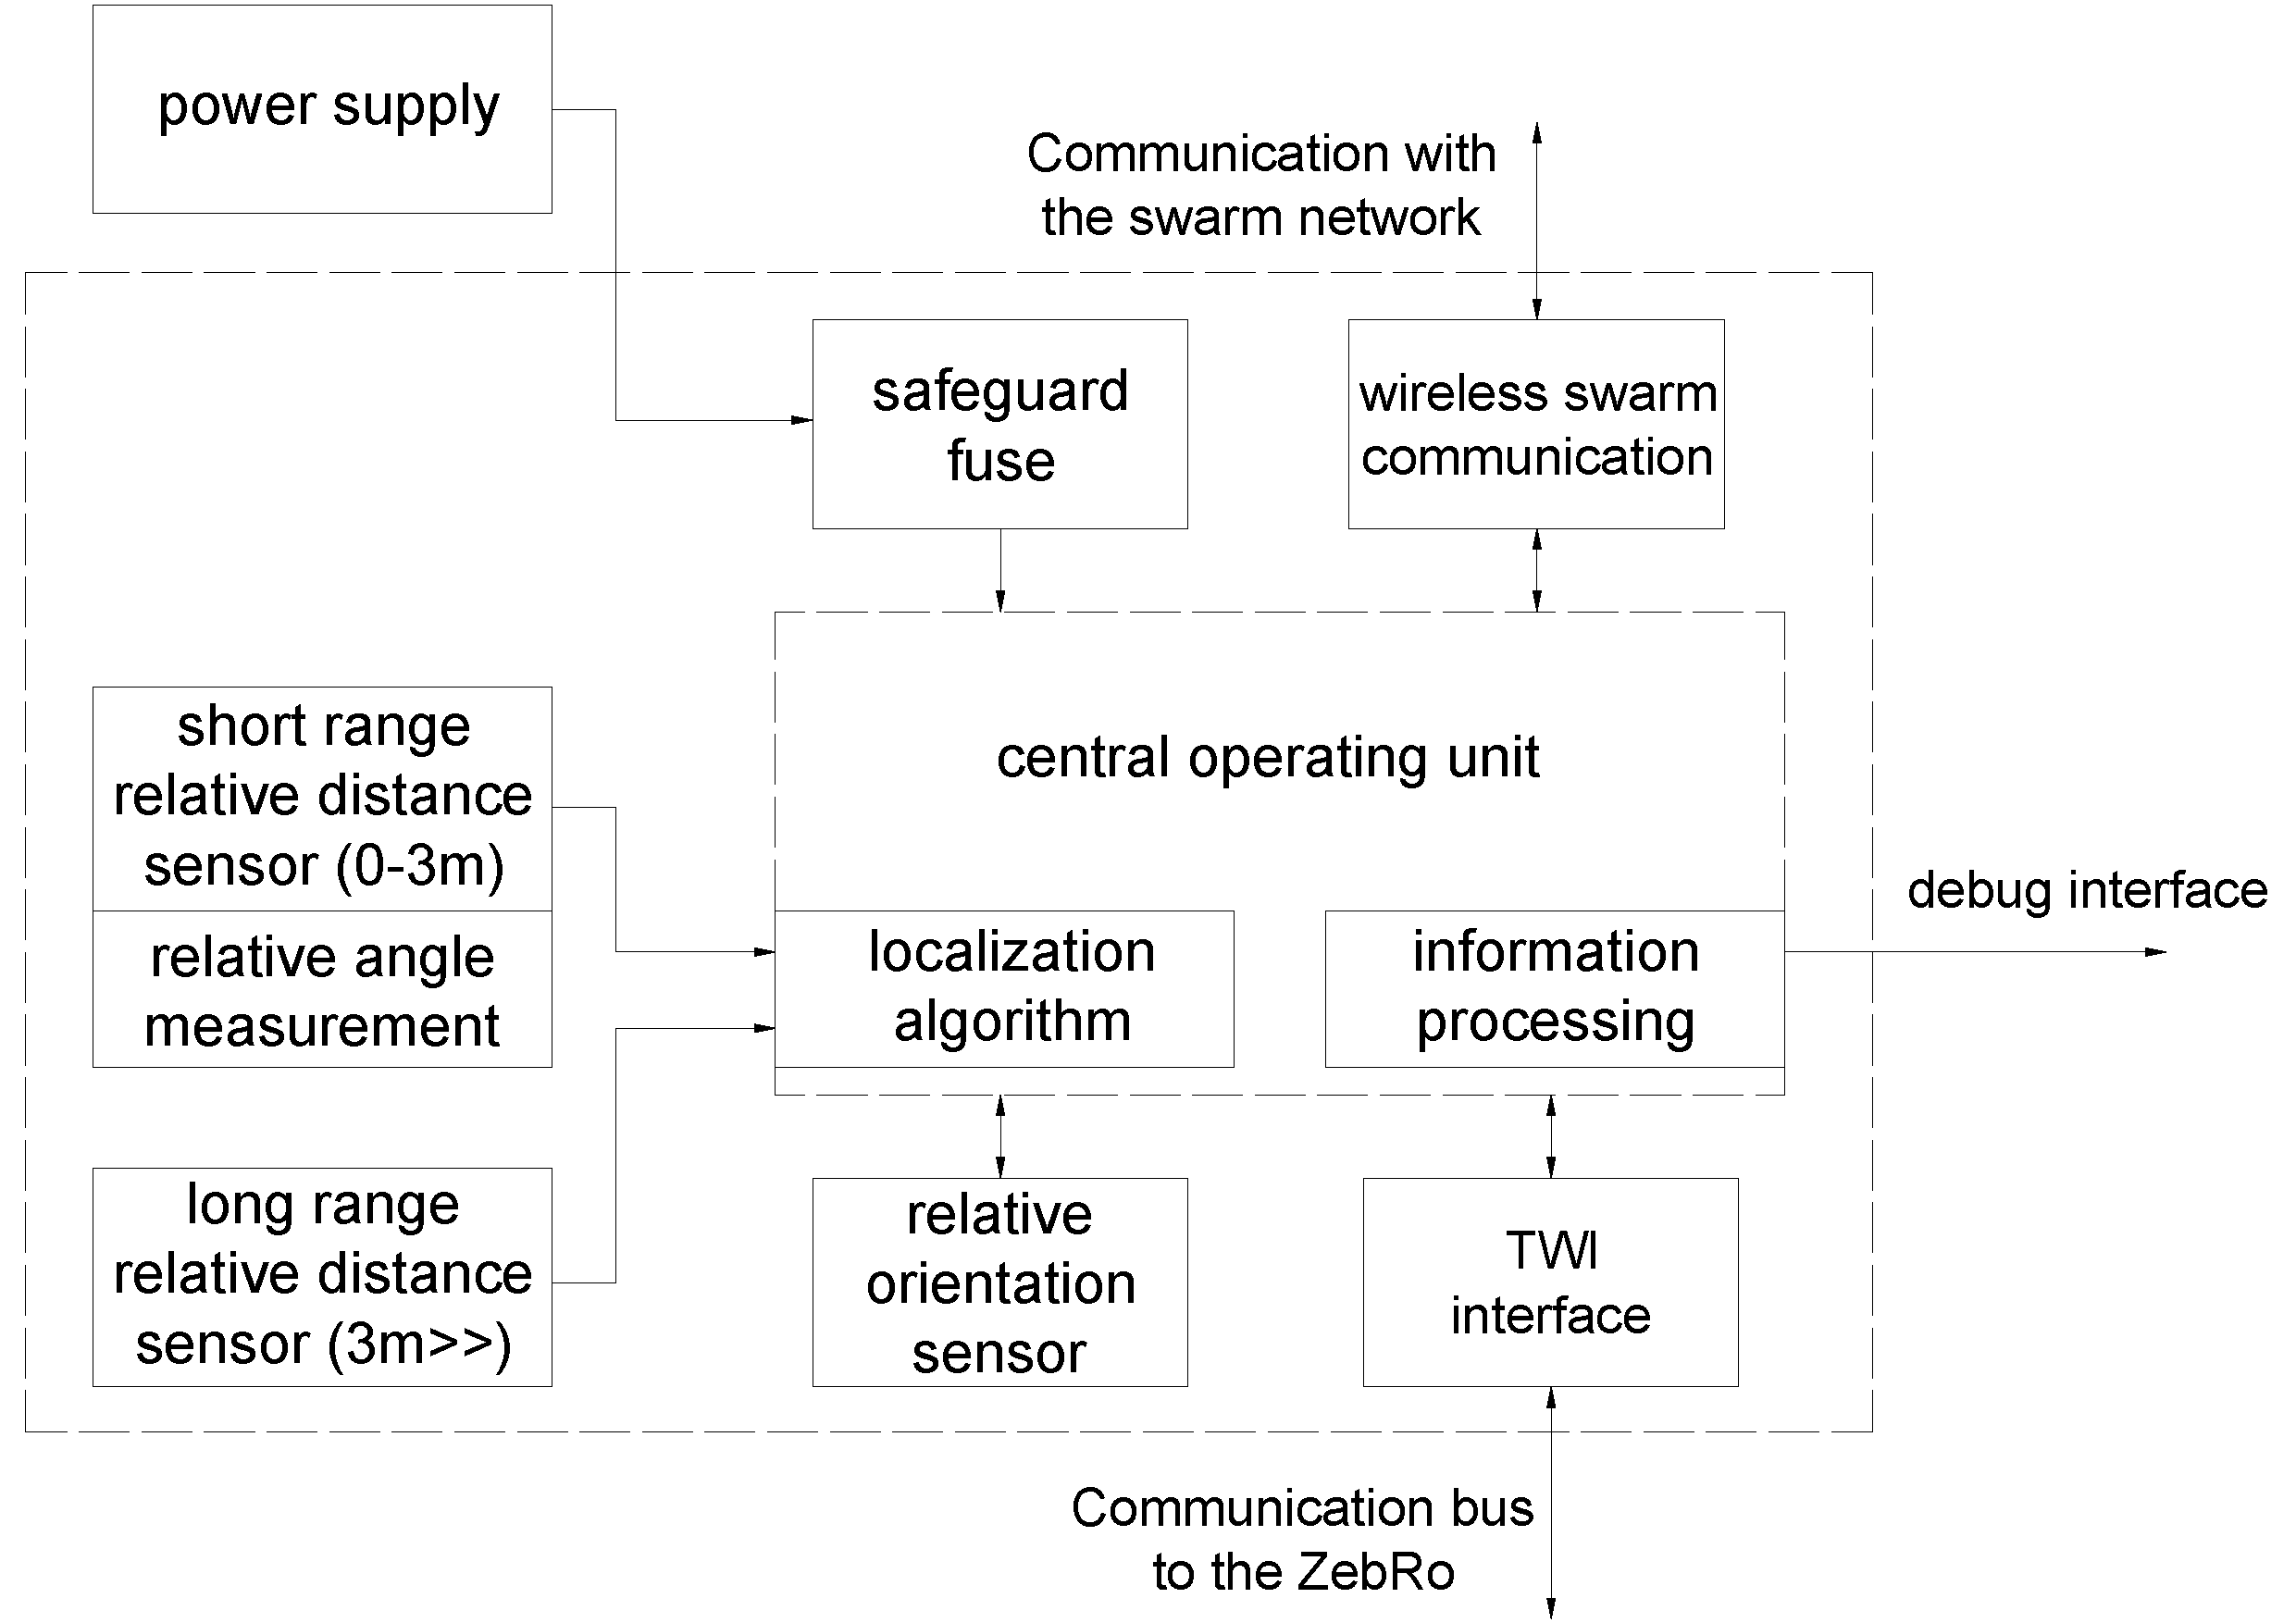
\includegraphics[width=1\textwidth]{overall.pdf}
  \caption{Overview of the swarm module design}
  \label{overall}
\end{figure}

\subsection{Short range localisation sensor}
The principle of the short range localisation sensor is displayed in figure \ref{demodulator} and \ref{modulator}.



As mentioned earlier the short relative distance measurement will be done acoustically. With acoustic sensing it is required to let the speaker sway to the right oscillation frequency, reaching this oscillation frequency takes time since the speaker won’t oscillate at the right frequency instantly. This complicates the measurement a little bit, since just detecting the to be measured signal won’t always translate into an exact distance due to the time the speakers take to sway into oscillation.

A solution to this problem is to create a fixed reference point within the sent signal. Creating this reference point after a fixed time enables the speaker to sway into oscillation making sure that no faulty measurements occur do to this “swaying time”. When the reference point has been detected by the receiver an accurate distance can be determined by subtracting the fixed “sway time”.

Without the implementation of this fixed reference point it is possible for a receiver to miss a few periods of the signal, due to the speaker still swaying into oscillation and the time of swaying being unknown. For example take an acoustic signal (Speed of sound 340.29 m/s) with a frequency of 4000Hz, one period of this signal is 0.00025s. Missing one period of this signal translates into a distance error of 8.5cm. Since the sway time of a speaker can change over time due to mechanical stresses a fixed time stamp seems the most suitable solution for the long term. The best way to create this reference point it still to be determined. This will be done by either frequency shift keying or phase shift modulation. Some real like testing will have to determine the best method.

\subsubsection{Modulation}
The modulation method is going to be determined by how well the reference point can be recognized by the demodulator. In the research phase, test were done with an speaker and a microphone. This showed that frequency and phase were well defined over distance but amplitude was not. Because of this the available methods for modulation of the acoustic signal are frequency modulation or phase modulation. The most important feature of the modulator must be consistency, meaning that the reference point should be send at exactly the same point in the signal every time. This is so that no deviation will occur when compensating for the missed periods before the reference point. In theory this can be done by both of the methods. 


See figure \ref{modulator} for a schematic representation of the modulator.

\begin{figure}[H]
  \centering
      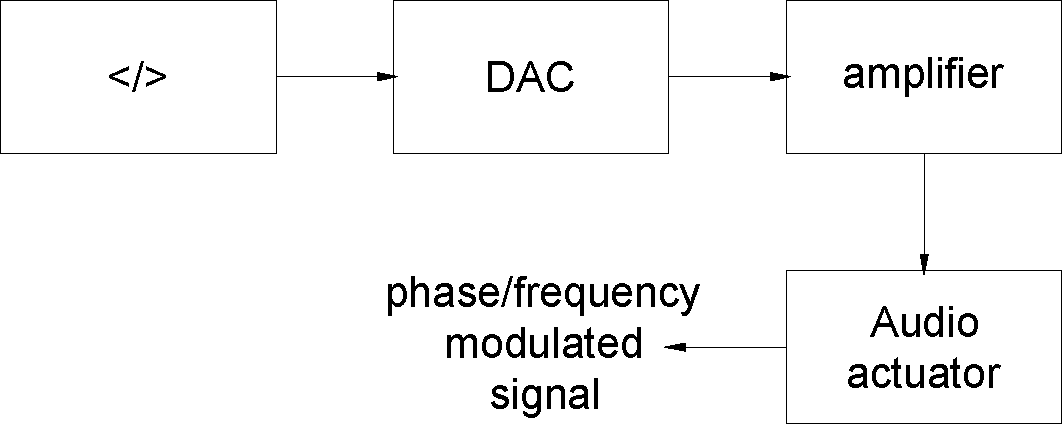
\includegraphics[width=0.8\textwidth]{modulator.pdf}
  \caption{Modulator}
  \label{modulator}
\end{figure}

\subsubsection{Demodulation}

A demodulator will be needed to retrieve the digital signal send from one swarm-module to another.  One swarming module will send an acoustic signal to the other modules, this signal will then be picked up by an sensor and will need to be processed properly before it can be used to determine the time it took the acoustic signal to travel from one swarming-module to the other. The signal retrieved by the acoustic sensor will also pick up a lot of noise and other sounds from the environment. Also, when further away the signal might be low in amplitude. To increase the amplitude and lower the noise, the signal will be amplified and filtered. These modifications to the signal will improve the signal to noise ratio drastically but a lot of noise might still remain. Therefore the demodulator itself must be insensitive to noise.  
The main purpose is the demodulator is to identify the reference point. And more importantly, determine the point in time the reference point is spotted. The time determined will be used to calculate the distance. Hence, the precision in which the demodulator determines the reference point in time effects the precision of the distance measurement. Only one swarming module will be sending his acoustic signal at any moment. When there are 10 units in its specified range and a preferred update frequency of 40Hz (see section 1). This gives every swarming-module only a small window in time to send their signal and for the other to receive it. When a frequency of 4kHz is chosen for the signal, every swarming-module will have 10 periods to send their signal. There for the demodulator must be able to lock onto the signal and determine the reference point within a few periods of the acoustic signal. See figure \ref{demodulator} for a schematic representation of the demodulator.

\begin{table}[H]
\centering
\caption{Demodulation specifications}
\label{demosensor}
\begin{tabular}{|p{1,5cm}|p{9,5cm}|}
\hline
Module   & Demodulator                                   \\ \hline
Input    & FSK Signal                                             \\ \hline
Outputs  & Reference point                                         \\ \hline
Function & Demodulation, Reference point detection \\ \hline
Features & Noise insensitive, precision (time), Quick demodulation  \\ \hline
\end{tabular}
\end{table}

\begin{figure}[H]
  \centering
      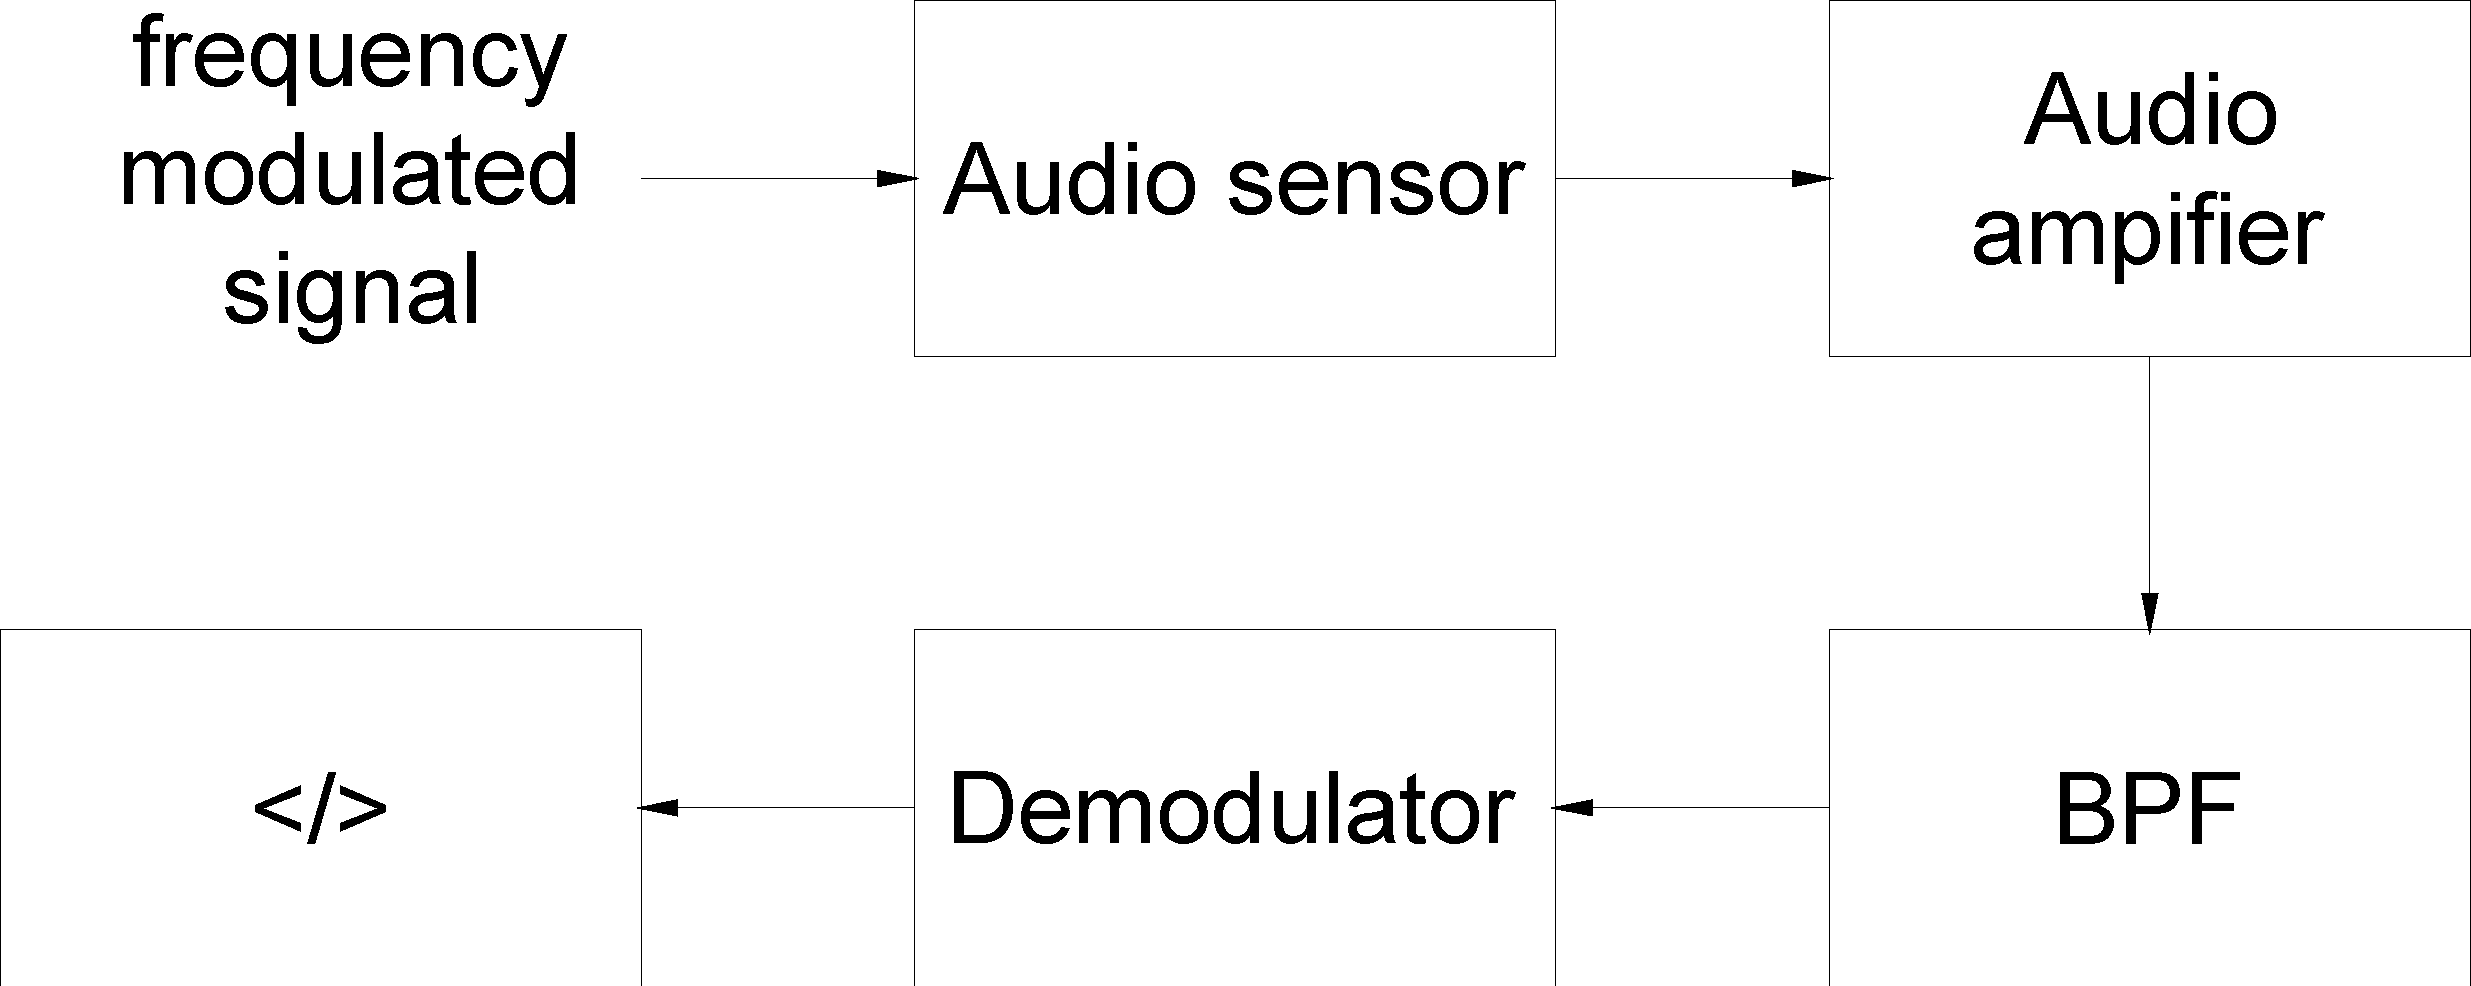
\includegraphics[width=1\textwidth]{demodulator.pdf}
  \caption{Demodulator}
  \label{demodulator}
\end{figure}





\section{Implementation}
Now that specifications of the functional blocks are defined, a implementation for these blocks will be found, using the information from our research. Just like section Functional specifications every block will be discussed independently. How all of the functional blocks fit together will be discussed in the section for the central processing unit.

\subsection{Short range localization sensor}
The short range localization consist of multiple smaller parts: Acoustic actuator/sensor, modulation/demodulation, distance measurement, and angle algorithm. 

\subsubsection{Acoustic actuator sensor}
As stated earlier a short range localization will be implemented using acoustic wave signals. The sensor will be implemented using microphones and an actuator will be implemented using a speaker. 

For Trigonometry angle determination the module must atleast poses three microphones spread in a triangle where all sides have the same distance as shown in figure \ref{module}.

For the distance between the different microphones a length of 10 cm is chosen because with the velocity propagation of sound being 343.2 m/s (at 20\degree C Celsius) and the underlying distance between de microphones being 10 cm using an 32 MHz micro-controller should grant enough overhead time to process the three different times being detected by the microphones. 

\begin{figure}[H]
\centering
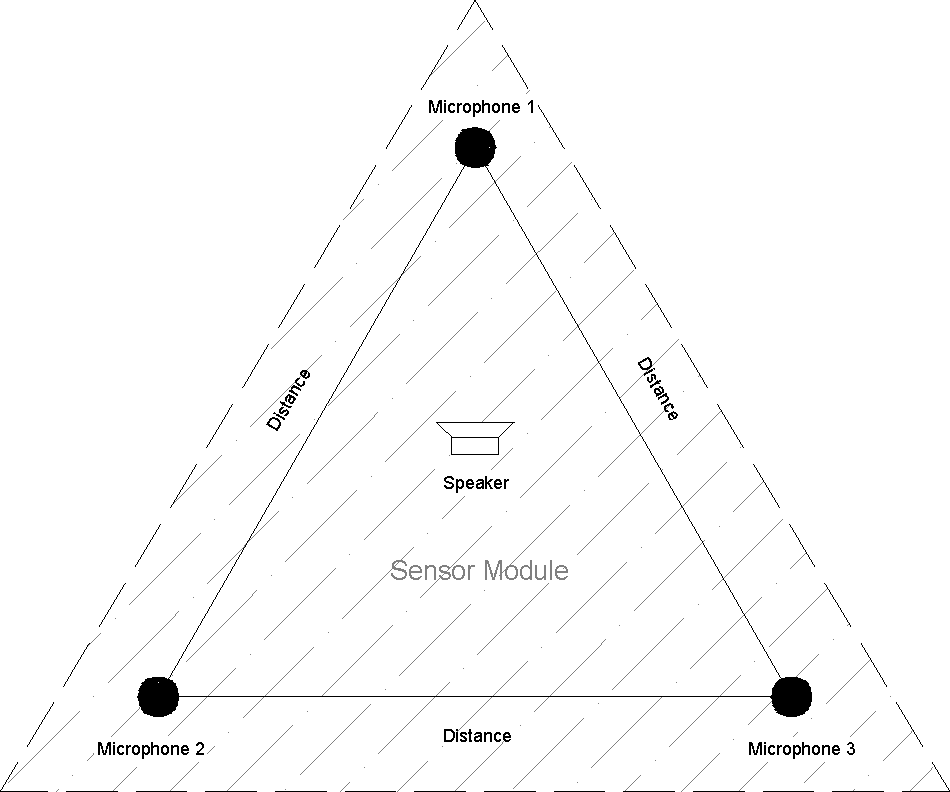
\includegraphics[width=1\textwidth]{Module.pdf}
\caption{Localization Module}
\label{module}
\end{figure}

The acoustic signal is send by a speaker facing upward. A metal plate is placed a 3 mm above the speaker, tests during the research phase showed this greatly improved the omnidirectional spread of the signal. The signal that's send it chosen to have a frequency of 4 kHz which has the best omnidirectional and range properties (section 4 of the research document).


The signal received by the microphone, translates in just a few millivolts. This signal is amplified for a total of 9600 by several stages of amplifiers, so that the signal clips on the supply voltage. This ruins the shape of the signal. However we're only interested in the frequency which will remain the same. After that the signal is bandpass filtered, to get rid of most of the noise. After this the signal is fed into the ADC of the Xmega128a4u. The modulator and demodulator will now be discussed in detail.\\\\
\textbf{Modulator}\\
The DAC of the Xmega128a4u is used to create a 4 kHz square wave signal. The signal will be send out for a pre-defined period of time and then the signal will pause for one period and continue. The pause will be the reference signal. The reference point is to eliminate certain uncertainties like the time it takes for the speaker to start resonating. The signal send looks like this 10 periods of signal, 2 periods nothing 10 periods of signal.\\ \textbf{ADD block diagram of modulator}\\\\
\textbf{Demodulator}
The demodulator has to be able to detect the frequency of the incoming signal. The demodulator has to differentiate between the wanted signal and other signal coming from the environment. This is done by looking at the characteristics of the signal, most importantly the frequency. The comparator in the ADC of the Xmega is used to count how many times the signal crosses a certain threshold. The frequency is derived from the simple fact that two crossings, should mean one period has passed. The reference-point is found when the micro-controller detect the send-pause-send sequence that's send by the modulator. Important to note is that the micro-controller looks at the time of the pause moment to make sure its the actual signal.\\
\textbf{ADD block diagram of demodulator} 

\subsubsection{Distance measurement}
The distance is derived from the time it takes the acoustic signal to travel from module A to module B. 
Suppose that module A is about to send its signal. Just before it starts sending the acoustic signal, it sends a message over the radio communication, which is almost instant compared to the speed of the sound waves. Module B starts its timer and wait for the signal to arrive. When it arrives it stops it's timer and takes off some pre-defined corrections based on tests done earlier. The distance can now be derived multiplying the speed of sound with the measured time.
\textbf{ADD state-diagram distance measurement}

\subsubsection{Angle measurement}
The Swarming module has three microphones placed with known distances between them. The relative angle is derived from the time measured with each microphone, and the distance between the microphones. In section 3.2 there's more information on how this is done.

The following algorithm shows pseudo-code how the angle will be calculated.
\lstinputlisting[firstline=1,lastline=40,label=code:locationalgo,caption=Algorithm to detect the location]{./code/Location_algorithm.c}




\section{Bibliografie}
\bibliography{references}
\bibliographystyle{IEEEtran}



\end{document}
